\chapter{Justificativa da abordagem}

\section{Considerações para escolha da abordagem}

São várias as metodologias aplicadas em desenvolvimento de software, cada uma com suas diferenças e vantagens a depender do projeto em que será aplicada.
Para realizar a comparação entre essas metodologias e escolher uma para ser aplicada há diversos critérios que podem ser utilizados, o autor Cockburn (2000) baseia-se em seis critérios: 
\begin{enumerate}       
\item Tamanho da equipe
\item O quão crítico é o sistema
\item Tamanho do projeto, da metodologia e do problema
\item Comunicação na equipe
\item Prioridades do projeto
\item Experiências anteriores
\end{enumerate}
    
\subsection{Tamanho da equipe}

    Como cita Cockburn, “A larger team needs a larger methodology”, com isso deve se levar em conta o tamanho da sua equipe, não se espera que metodologias para times pequenos vá funcionar em times maiores, porque pode haver falha de comunicação, e esperar que metodologias para times maiores funcione em seu total desempenho com times pequenos.

\subsection{O quão crítico é o sistema}

    Analisar no que falhas no sistema podem gerar como resultado, ou o quanto as pessoas dependem do sucesso desse software, Cockburn (2000) divide sistemas críticos em quatro zonas de perda:
\begin{itemize}
\item Perda de conforto: acontece quando as falhas no sistema apenas geram desconforto as pessoas que estão utilizando do mesmo, gerando trabalho braçal para o usuário ou retrabalho desnecessário.

\item Perda de verbas discricionárias: acontece quando as falhas de sistema acarretam em perda de dinheiro de uma forma mais discreta, só no alcance do desconforto.

\item Perda de verbas insubstituíveis: sugere que a perda de verbas pode gerar uma crise na empresa podendo acarretar falência.

\item Perda de vidas: sugere que a vida das pessoas corre risco, caso o sistema tenha mal funcionamento.

\item Com essas quatro zonas, pode-se verificar que sistemas críticos justificam o uso de metodologias que exigem mais documentação e também mais gastos para que a segurança do produto não seja violada e venha gerar essas zonas de perda.
\end{itemize}

\subsection{Tamanho do projeto, da metodologia e do problema}

    Como Cockburn (2000) cita, “incrementar o tamanho ou densidade da metodologia pode acarretar mais custo de tempo e dinheiro”. Esse princípio aborda custos envolvidos à adição de elementos e controle da equipe na metodologia.
    Por exemplo, ter um projeto muito grande e trabalhar com metodologias aplicadas para equipes pequenas pode dar certo, mas vai gerar muito mais trabalho para essas pessoas além de aumentar o custo do projeto, com isso deve-se basear nas características do projeto, como tamanho e complexidade para resolver o problema, para definir a metodologia a ser utilizada.
        
\begin{figure}[!htpb]
\centering
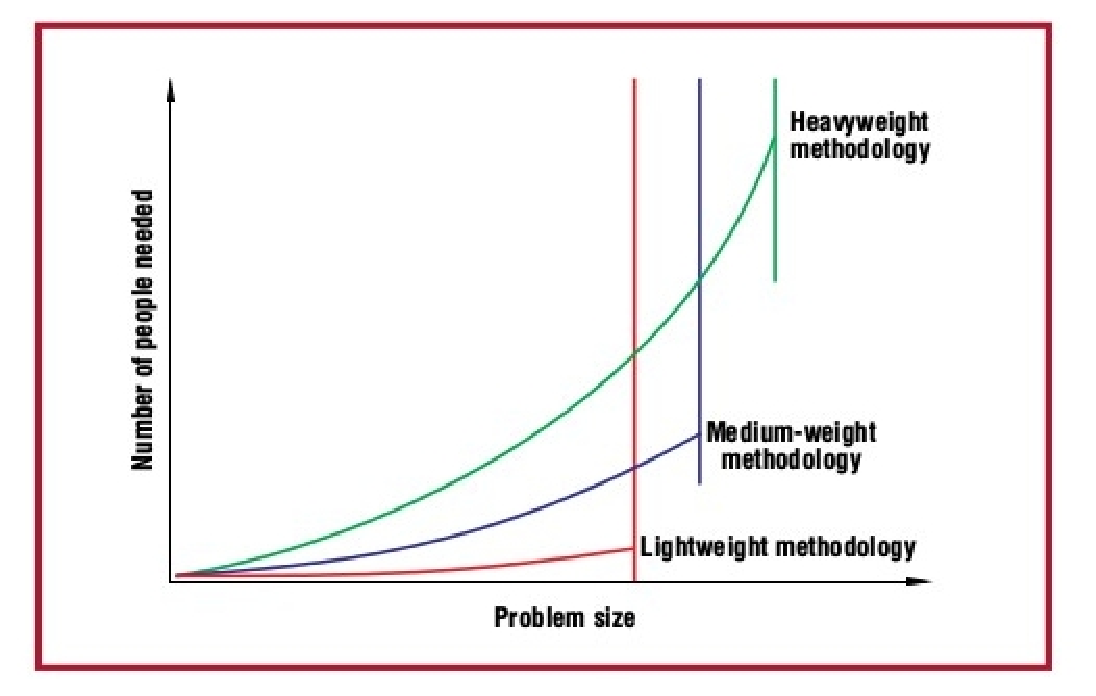
\includegraphics[scale=0.8]{figuras/abordagem/cockburngraph}
\caption{Gráfico de relação entre tamanho de projeto, metodologia, problema}
\end{figure}

\subsection{Comunicação da equipe}

    Este princípio aborda a interação entre a equipe, deve-se considerar alguns aspectos como o tamanho da equipe e proximidade na hora de realizar o trabalho necessário, por exemplo, se a equipe é pequena e pode se comunicar pessoalmente de forma diária, prefere-se usar uma abordagem ágil, agora se a equipe consiste em um grande número de pessoas, trabalhando de uma forma que a comunicação se dê por trocas de e-mails, videoconferências, entre outros, espera-se que seja escolhida uma abordagem tradicional.

\subsection{Prioridades do projeto}
Analisar questões como o deadline de entrega do projeto, visibilidade de produção ou requisição de documentação são aspectos abordados nesse critério. Todos esses aspectos influenciam na escolha da metodologia, por exemplo se o cliente preza mais pelo produto funcionando do que documentação relatando o software, adota-se uma abordagem ágil.

\subsection{Experiências anteriores}

Fazer uma análise das experiências anteriores da equipe em relação a atuação em projetos com diferentes tipos de metodologias, e ver em qual a mesma foi mais produtiva ou se identificou mais para trabalhar.


\subsection{Perfil do cliente}
Além desses aspectos definidos por Cockburn (2000) a equipe resolveu abordar alguns aspectos a mais voltados ao cliente, como a formalidade e disponibilidade do mesmo para execução de reuniões, além do tamanho do contexto do problema que se trata do controle de estoque e desperdício.


\section{A escolha da metodologia}

    A equipe preferiu adotar uma abordagem ágil devido ao contexto observado, e ao seguir os aspectos apresentados por Cockburn (2000) aplicados à situação, que será justificado logo abaixo:
\begin{itemize}
\item O fato de a equipe ter apenas quatro pessoas, a faz ser pequena, justificando a escolha de uma metodologia aplicada a equipes pequenas, atendendo ao primeiro critério.
\item O sistema a ser construído é para controle de desperdício e estoque, não se tornando um sistema tão crítico, que pode ferir duas das zonas de perdas, mas são as mais leves, a referente a perda de conforto pelo fato de o que já está sendo feito na padaria que é um trabalho manual para controlar tais situações de desperdício e estoque, e a perda de verbas discricionárias referente a um mau funcionamento do sistema que poderia acarretar perda de alguns fundos voltados à mercadoria.
\item O problema a ser resolvido não é tão complexo, fazendo com que o projeto para solucioná-lo apresente uma solução eficiente, mas não tão difícil de ser executada, também foi levado em conta que o prazo da entrega do software é bem curto. Com isso foi mais interessante escolher a abordagem ágil.
\item Outro critério observado, foi que a equipe consegue se encontrar facilmente para realização de rituais da metodologia ágil, como comunicação pessoal diariamente devido a grande semelhança entre as grades horárias dos integrantes da equipe.
\item Em relação a prioridade do projeto, o cliente busca um software para atender a demanda que ele exigiu, que é controle de estoque e desperdício, e por se tratar de um negócio mais familiar não exigiu a documentação de características do software.
\item A equipe se sentiu mais à vontade trabalhando com a metodologia ágil em experiências anteriores, pelo fato da proximidade da equipe ser um fator importante, além de prezar pelo funcionamento do produto.

\item O cliente citou que o negócio se trata de um investimento familiar, o mesmo também se encontra bastante disponível para a realização de reuniões. Além de não exigir tanta formalidade em relação ao desenvolvimento do projeto.
\end{itemize}